\documentclass[12pt,a4paper]{article}
\usepackage[utf8]{inputenc}
\usepackage[russian]{babel}
\usepackage{amsmath}
\usepackage{amsfonts}
\usepackage{amssymb}
\usepackage[left=2cm,right=2cm,top=2cm,bottom=2cm]{geometry}
\usepackage{graphicx}
\begin{document}
Контрольная работа номер 3. 19.03.2014. 

\begin{figure}[hbtp]
\centering
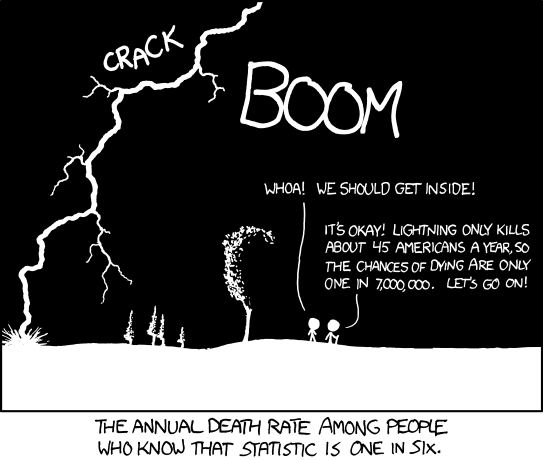
\includegraphics[scale=0.7]{stats.png}
\end{figure}



\begin{enumerate}
\item Дед Мазай подбирает зайцев. Предположим, что длина левого уха зайца имеет экспоненциальное распределение с плотностью $f(x)=a\exp(-ax)$ при $x\geq 0$. По 100 зайцам оказалось, что $\sum x_i=2000$. 
\begin{enumerate}
\item  Найдите оценку $\hat{a}$ методом моментов
\item Оцените стандартную ошибку $se(\hat{a})$
\item Постройте 90\%-ый доверительный интервал для неизвестного $a$
\item На уровне значимости $\alpha=0.05$ проверьте гипотезу $H_0$: $a=15$ против $a>15$. Найдите точное P-значение.
\end{enumerate}

\item По совету Лисы Волк опустил в прорубь хвост и поймал 100 чудо-рыб. Веса рыбин независимы и имеют распределение Вейбулла, $f(x)=2\exp(-x^2/a^2)\cdot x/a^2$ при $x\geq 0$. Известно, что $\sum x_i^2=120$.
\begin{enumerate}
\item  Найдите оценку $\hat{a}$ методом максимального правдоподобия
\item Оцените стандартную ошибку $se(\hat{a})$
\item Постройте 90\%-ый доверительный интервал для неизвестного $a$
\item На уровне значимости $\alpha=0.05$ проверьте гипотезу $H_0$: $a=1$ против $a>1$. Найдите точное P-значение.
\end{enumerate}


\item $[$R] Как известно, Фрекен-Бок пьет коньяк по утрам и иногда видит привидения. За 110 дней имеются следующие статистические данные


\begin{tabular}{c|ccc}
Рюмок & 1 & 2 & 3 \\ 
\hline 
Дней с привидениями & 10 & 25 & 20 \\ 
Дней без привидений & 20 &  25 & 10 \\ 
\end{tabular}

Вероятность увидеть привидение зависит от того, сколько рюмок коньяка было выпито утром, а именно, $p=\exp(a+bx)/(1+ \exp(a+bx))$, где $x$ --- количество рюмок, а $a$ и $b$ --- неизвестные параметры.

\begin{enumerate}
\item Оцените неизвестные параметры с помощью максимального правдоподобия.
\item На уровне значимости $\alpha=0.05$ помощью теста отношения правдоподобия проверьте гипотезу о том, что одновременно $a=0$ и $b=0$. В чем содержательный смысл этой гипотезы? Найдите точное P-значение.
\end{enumerate}


%\item Иванушка-дурачок поймал 500 жар-птиц, взвесил и отпустил. Предположим, что веса жар-птиц независимы и имеют гамма-распределение с функцией плотности $f(x)=\lambda^k x^{k-1}\exp(-\lambda x)/ \Gamma(k)$ при $x\geq 0 $. Известно, что $\sum x_i=900$, a $\sum \ln x_i =200$. Логарифм гамма-функции, $\ln \Gamma(k)$, реализуется в R командой \verb|lgamma(k)|.
%\begin{enumerate}
%\item Оцените параметры гамма-распределения с помощью максимального правдоподобия.
%\item На уровне значимости $\alpha=0.05$ помощью теста отношения правдоподобия проверьте гипотезу о том, что одновременно $k=2$ и $\lambda=1$.
%\end{enumerate}


\item Кот Васька поймал 5 воробьев, взвесил и отпустил. Предположим, что веса воробьев независимы и имеют нормальное распределение $N(\mu,\sigma^2)$. Известно, что $\sum x_i=10$ и $\sum x_i^2=25$.
\begin{enumerate}
\item Постройте 90\% доверительный интервал для $\sigma^2$, симметричный по вероятности
\item $[$R]  Постройте самый короткий 90\% доверительный интервал для $\sigma^2$
\end{enumerate}


\item Задача о немецких танках. Всего выпущено неизвестное количество $n$ танков. Для упрощения предположим, что на каждом танке написан его порядковый номер\footnote{В реальности во время Второй мировой войны при оценке количества танков <<Пантера>> выпущенных в феврале 1944 использовались номера колес. Двух подбитых танков оказалось достаточно, чтобы оценить выпуск в 270 танков. По немецким архивам фактический объем выпуска оказался равен 276 танков. }. В бою было подбиты 4 танка с номерами 2, 5, 7 и 12. 
\begin{enumerate}
\item Найдите оценку общего выпуска танков $n$ с помощью метода максимального правдоподобия
\item Является ли оценка максимального правдоподобия несмещенной?
\item Является ли максимум из номеров подбитых танков достаточной статистикой?
\item Является ли максимум из номеров подбитых танков полной статистикой?
\item Постройте с помощью оценки максимального правдоподобия несмещенную эффективную оценку неизвестного $n$.
\end{enumerate}

\item Гражданин Фёдор решает проверить, не жульничает ли напёрсточник Афанасий, для чего предлагает Афанасию сыграть 5 партий в напёрстки. Фёдор решает, что в каждой партии будет выбирать один из трёх напёрстков наугад, не смотря на движения рук ведущего. Основная гипотеза: Афанасий честен, и вероятность правильно угадать напёрсток, под которым спрятан шарик, равна 1/3. Альтернативная гипотеза: Афанасий каким-то образом жульничает (например, незаметно прячет шарик), так что вероятность угадать нужный напёрсток меньше, чем 1/3. Статистический критерий: основная гипотеза отвергается, если Фёдор ни разу не угадает, где шарик.
\begin{enumerate}
\item Найдите уровень значимости критерия.
\item Найдите вероятность ошибки второго рода в том случае, когда Афанасий жульничает, так что вероятность угадать нужный напёрсток равна 1/5.
\end{enumerate}

\item $[$R] В службе единого окна 5 клиентских окошек. В каждое окошко стоит очередь. Я встал в очередь к окошку номер 5 ровно в 15:00, передо мной 5 человек. Предположим, что время обслуживания каждого клиента --- независимые экспоненциальные величины с параметром $\lambda$. Первый человек с момента моего прихода был обслужен в окошке 1 в 15:05. Второй человек с момента моего прихода был обслужен в окошке 2 в 15:10. 
\begin{enumerate}
\item Оцените с помощью максимального правдоподобия параметр $\lambda$
\item Оцените, сколько мне еще стоять в очереди.
\end{enumerate}

\end{enumerate}




\end{document}